% ~ 6 pages
\chapter{Machine Learning}
\label{sec:ml}

\todo[inline]{Make consistent usage of: Observation, example, event, item, etc.}

Machine learning is the study of algorithms that learn structure from data
(called training data) and can subsequently be used to make predictions on
unseen data. Examples for such algorithms are \emph{Boosted Decision Trees}
(BDT) and \emph{Neural Networks} (NN) which are able to model nonlinear problems
without the need to supply an explicitly derived rule-set or functional form.
They often offer superior performance compared to linear models or simple
cut-based approaches at the cost of interpretability. Machine learning
techniques are widely used in particle physics e.g.\ for the reconstruction of
hadronic tau decays in the ATLAS experiment. There they are used for tau
identification, track classification, decay mode classification, and energy
calibration.

The focus of this chapter lies on supervised learning, which is concerned with
learning models from labelled data (each example consisting of explanatory
variables and a dependent variable/label \todo{define and get rid of parens}).
This domain includes regression for modelling a continuous response and
classification for assigning class labels (e.g.\ signal or background) to an
observation with associated input variables. This chapter gives an overview of
the classification techniques used in this thesis starting with a brief
description of \emph{Boosted Decision Trees} that are used in
Chapter~\ref{sec:bdt} for rejection of tau candidates originating from dijet
events \todo{defined?}. A comprehensive summary on \emph{Recurrent Neural
  Networks} that are used for tau identification \todo{defined?} is given in
Chapter~\ref{sec:rnn} and additionally for decay mode classification in
Chapter~\ref{sec:decaymode}. The chapter is concluded with an overview of the
software frameworks used in this thesis.

\section{Boosted Decision Trees}
\label{sec:bdt}

\emph{Boosted Decision Trees} consist of an ensemble of decision trees that is
created by a meta-algorithm called \emph{boosting}. In
Section~\ref{sec:ml_decision_trees} the decision tree algorithm is presented. A
brief overview of \emph{boosting} algorithms is given in
Section~\ref{sec:ml_boosting}. The description focuses on binary classification
tasks aiming to discriminate between two distinct classes, hereafter called
signal and background.

\subsection{Decision Trees}
\label{sec:ml_decision_trees}

\begin{figure}[htb]
  \centering
  \begin{subfigure}[t]{0.4\textwidth}
    \centering
    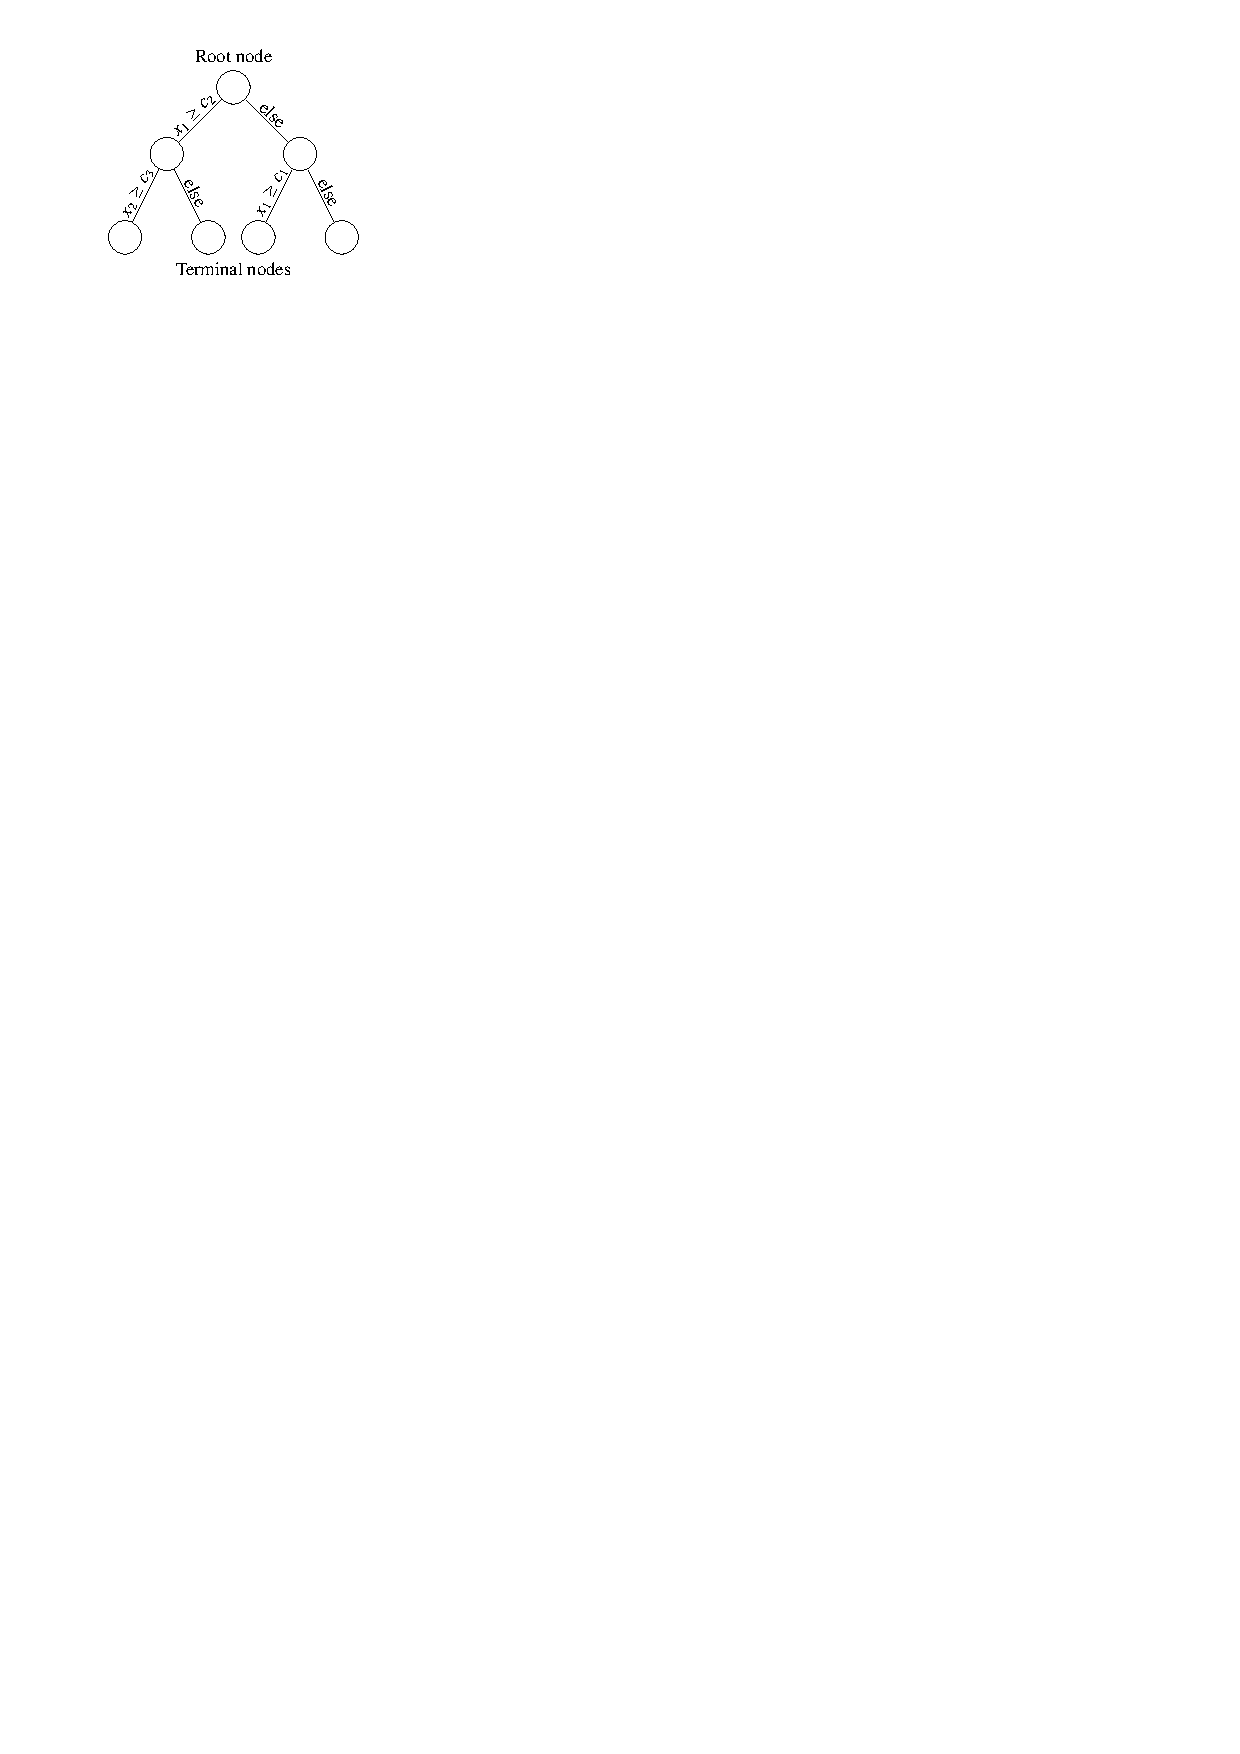
\includegraphics{./figures/theory/decision_tree.pdf}
    \subcaption{Binary tree structure of decision trees.}
    \label{fig:decision_tree_binary_tree}
  \end{subfigure}\hspace*{2em}
  \begin{subfigure}[t]{0.4\textwidth}
    \centering
    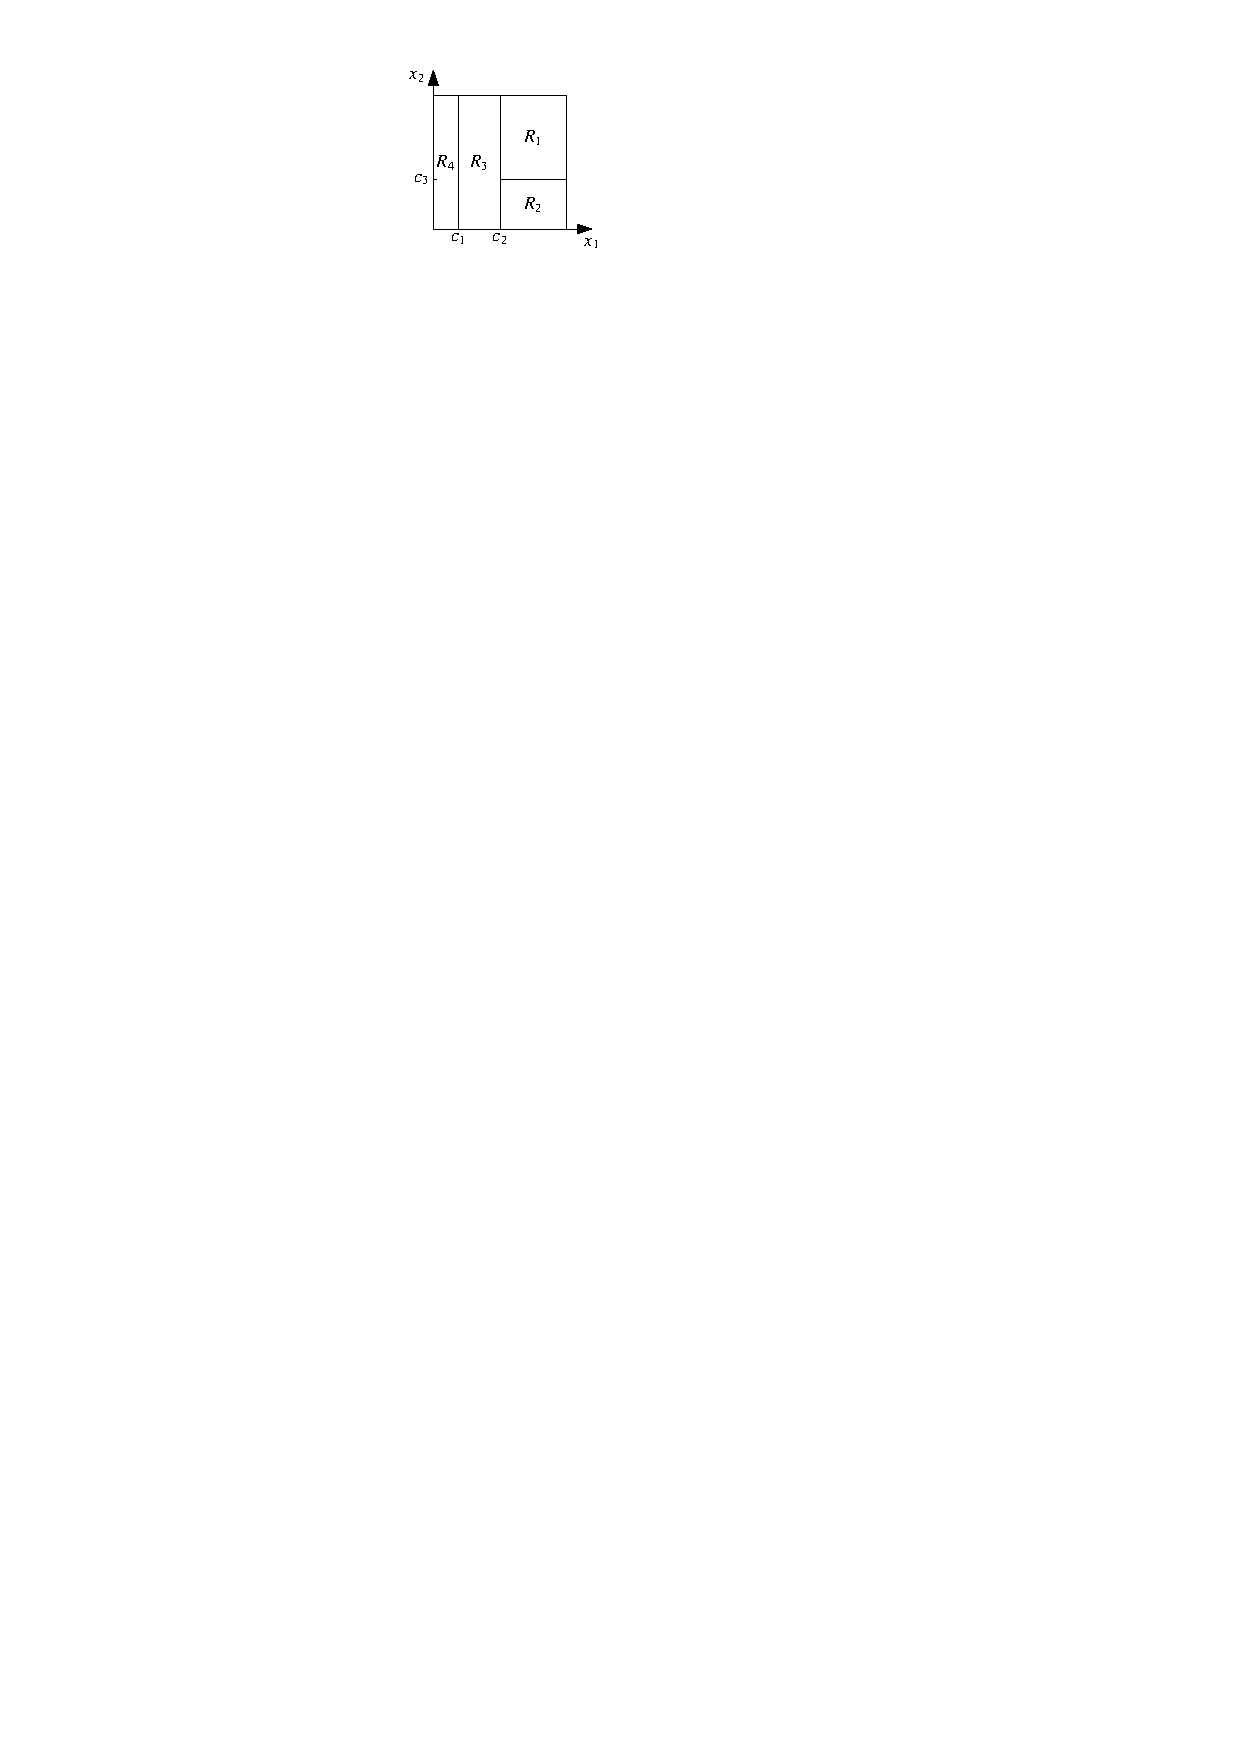
\includegraphics{./figures/theory/decision_tree_partition.pdf}
    \subcaption{Partitioning of the space spanned by the input variables $x_1$
      and $x_2$ into subregions~$R_i$.}
    \label{fig:decision_tree_partition}
  \end{subfigure}
  \caption{Structure of a decision tree with depth~$d_\text{tree} = 2$ and two
    input variables $x_1$, $x_2$. Adapted from Ref.~\cite{esl}.}
  \label{fig:decision_tree}
\end{figure}

A decision tree is a tree-based model that recursively partitions the space
spanned by the input variables into disjoint subregions by applying binary
splits on the coordinate axes until a stopping criterion is met. Frequently used
criteria include limiting the maximum depth of the tree or requiring a minimum
number of training examples in a subregion considered for further splitting.
Figure~\ref{fig:decision_tree_binary_tree} shows the binary tree structure of a
decision tree. The root node of the tree contains the entire dataset which is
subsequently split into two nodes by a condition on a single input variable. The
terminal nodes contain disjoint subsamples of the dataset with input variables
falling into the distinct regions of the variable space depicted in
Figure~\ref{fig:decision_tree_partition}. Observations \todo{Better word --
  item?} falling into a subregion are assigned the probability of being signal
given by the fraction of signal events (i.e.\ the signal purity) of the training
data in this region.
% Each terminal node is assigned the
% majority class of the subset of training data contained within it. An
% alternative method to gauge the confidence of the decision is to assign the
% signal purity.
% The subregions of the variable space defined by the terminal nodes Formally:
% majority class minimises classification error, signal purity minimises
% log-loss

A decision tree is grown using a greedy optimisation method, where each node is
split on the variable and value that gives the largest improvement according to
a chosen impurity measure. Commonly used for binary classification trees is the
\emph{Gini impurity} given by
\begin{align*}
  I_\text{G}(p) = 2 p (1 - p)
\end{align*}
where $p$ is the signal or background purity~\cite{esl} \todo{Define what
  impurity measure does?}. The best split is chosen such that the mean of the
Gini impurities of the resulting nodes, weighted by the sum of event weights in
each node, is minimised.
% Gini index: Probability to assign the correct label to a randommly picked
% observation when randomly assigning according to the distribution of labels in
% the sample

\subsection{Boosting}
\label{sec:ml_boosting}

Boosting describes a family of machine learning meta-algorithms that are used to
build ensembles of base learner aiming to improve the overall predictive power
compared to a single model. The ensembles can be viewed as an additive expansion
in a set of basis functions given by the base learner \cite{esl}. Boosting is
commonly used in conjunction with Decision Trees giving rise to so called
\emph{Boosted Decision Trees}.

Adaptive Boosting (\emph{AdaBoost}) is a boosting algorithm that forms a
weighted sum of a base classifier, where each classifier is trained on data that
is reweighted such that training examples \todo{consistent wording} that were
previously incorrectly classified contribute with higher weight than examples
\todo{consistent wording} that were correctly classified. A generalisation of
this method is called \emph{gradient boosting} which minimises the expected
value of an arbitrary differential loss function (i.e.\ a function penalising
errors of the model) during boosting. Gradient boosting reproduces the
\emph{AdaBoost} algorithm if the exponential loss function
\begin{align*}
  L\left(y, f(\mathbf{x})\right) = \exp\left(- y f(\mathbf{x})\right)
\end{align*}
with input variables~$\mathbf{x}$, true class~$y \in \{ -1, 1 \}$ and model
response~$f(\mathbf{x}) \in [-1, 1]$ \todo{mapped into this interval} for a
given event is used~\cite{esl}. For general loss functions no convenient methods
for minimising the loss exist and a gradient descent algorithm is used. A full
mathematical description of the algorithm is omitted for brevity and can be
found in Ref.~\cite{friedman_gbm, esl}. In this thesis gradient boosting with
the loss function
\begin{align*}
  L\left(y, f(\mathbf{x})\right) = \log\left( 1 + \exp(- 2 y f(\mathbf{x})) \right)
\end{align*}
is used, which is empirically shown to be less susceptible to noise
\todo{features originating from statistical fluctuations} and outliers (i.e.\
examples with large negative margins~$y f(\mathbf{x})$) than \emph{AdaBoost}
\cite{esl, schapire_boosting}.
% The reason is that the
% exponential loss applies a larger penalty to training examples with large
% negative margins~$y f(x)$, e.g.\ outliers.
%
% (called \emph{LogitBoost}~\cite{logitboost})

\section{Artificial Neural Networks}
\label{sec:nn}

Artificial neural networks encompass a large set of models that can be used as
approximations to a wide variety of nonlinear functions \cite{hornik}. They can
be thought of as rules to compute a
mapping~\mbox{$\mathbb{R}^n \rightarrow \mathbb{R}^m$} between a set of
$n$~input variables and $m$~desired responses. The central idea is to repeatedly
compute intermediate representations of the inputs by applying transformations
and combining the final representation in a linear or logistic regression model.
Neural networks are typically organised into different \emph{layers} defining
the transformation that is applied on the layer inputs. Multiple layers
connected according to a computational graph form a network. This scheme allows
for great flexibility in building different models making neural networks
prevalent in many areas of machine learning research~\cite{goodfellow_dl}.

The following sections introduce concepts needed to understand the models used
for the classification tasks in this thesis. Matrices are denoted using
uppercase and vectors using lowercase bold symbols e.g.\ input
variables~$\mathbf{x}$ and weight matrices~$\mathbf{W}$.

\subsection{Feedforward Neural Networks}
\label{sec:nn_feedforward}
Feedforward neural networks are networks in which information flows strictly in
the forward direction, disallowing feedback loops between input and output of a
single layer. An example of simple feedforward neural networks are the so called
\emph{multi-layer perceptrons}. They consist of a number of input neurons
$\mathbf{x}$, which are used to pass the discriminating variables to the
network, and an output layer with neuron activations~$\mathbf{y}$ after applying
a nonlinear activation function to the values of the neurons. The input and
output layers are connected by one or more intermediate hidden layers.
\begin{figure}[htb]
  \centering
  \begin{minipage}[t]{0.55\textwidth}
    \centering
    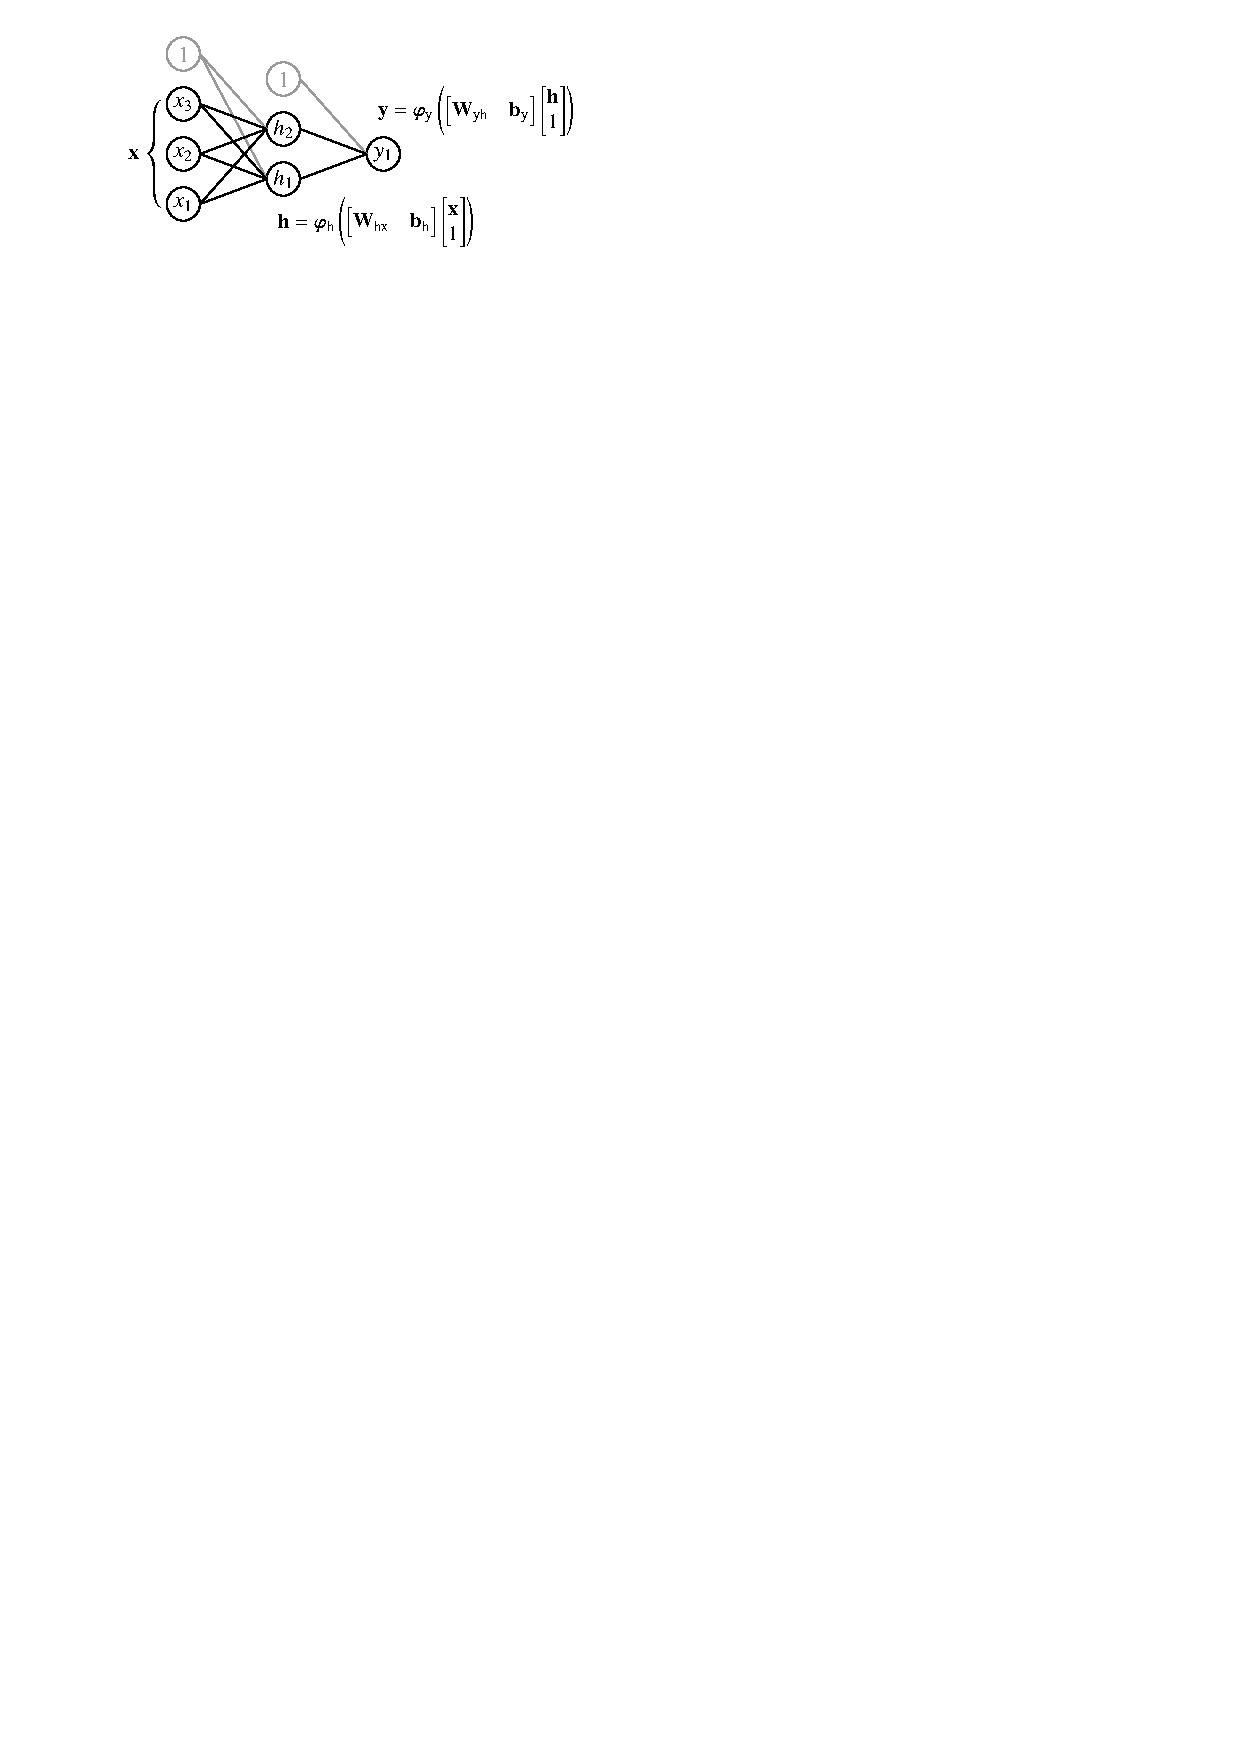
\includegraphics{./figures/theory/mlp.pdf}
    \captionof{figure}{Multi-layer perceptron with input layer~$\mathbf{x}$,
      hidden layer~$\mathbf{h}$ and output layer~$\mathbf{y}$. Activations are
      given after applying an element-wise activation function~$\bm{\varphi}$.
      Block matrix notation is used to indicate how biases~$\mathbf{b}$ can be
      absorbed into a single weight matrix.}
    \label{fig:multi_layer_perceptron}
  \end{minipage}\hfill
  \begin{minipage}[t]{0.4\textwidth}
    \centering
    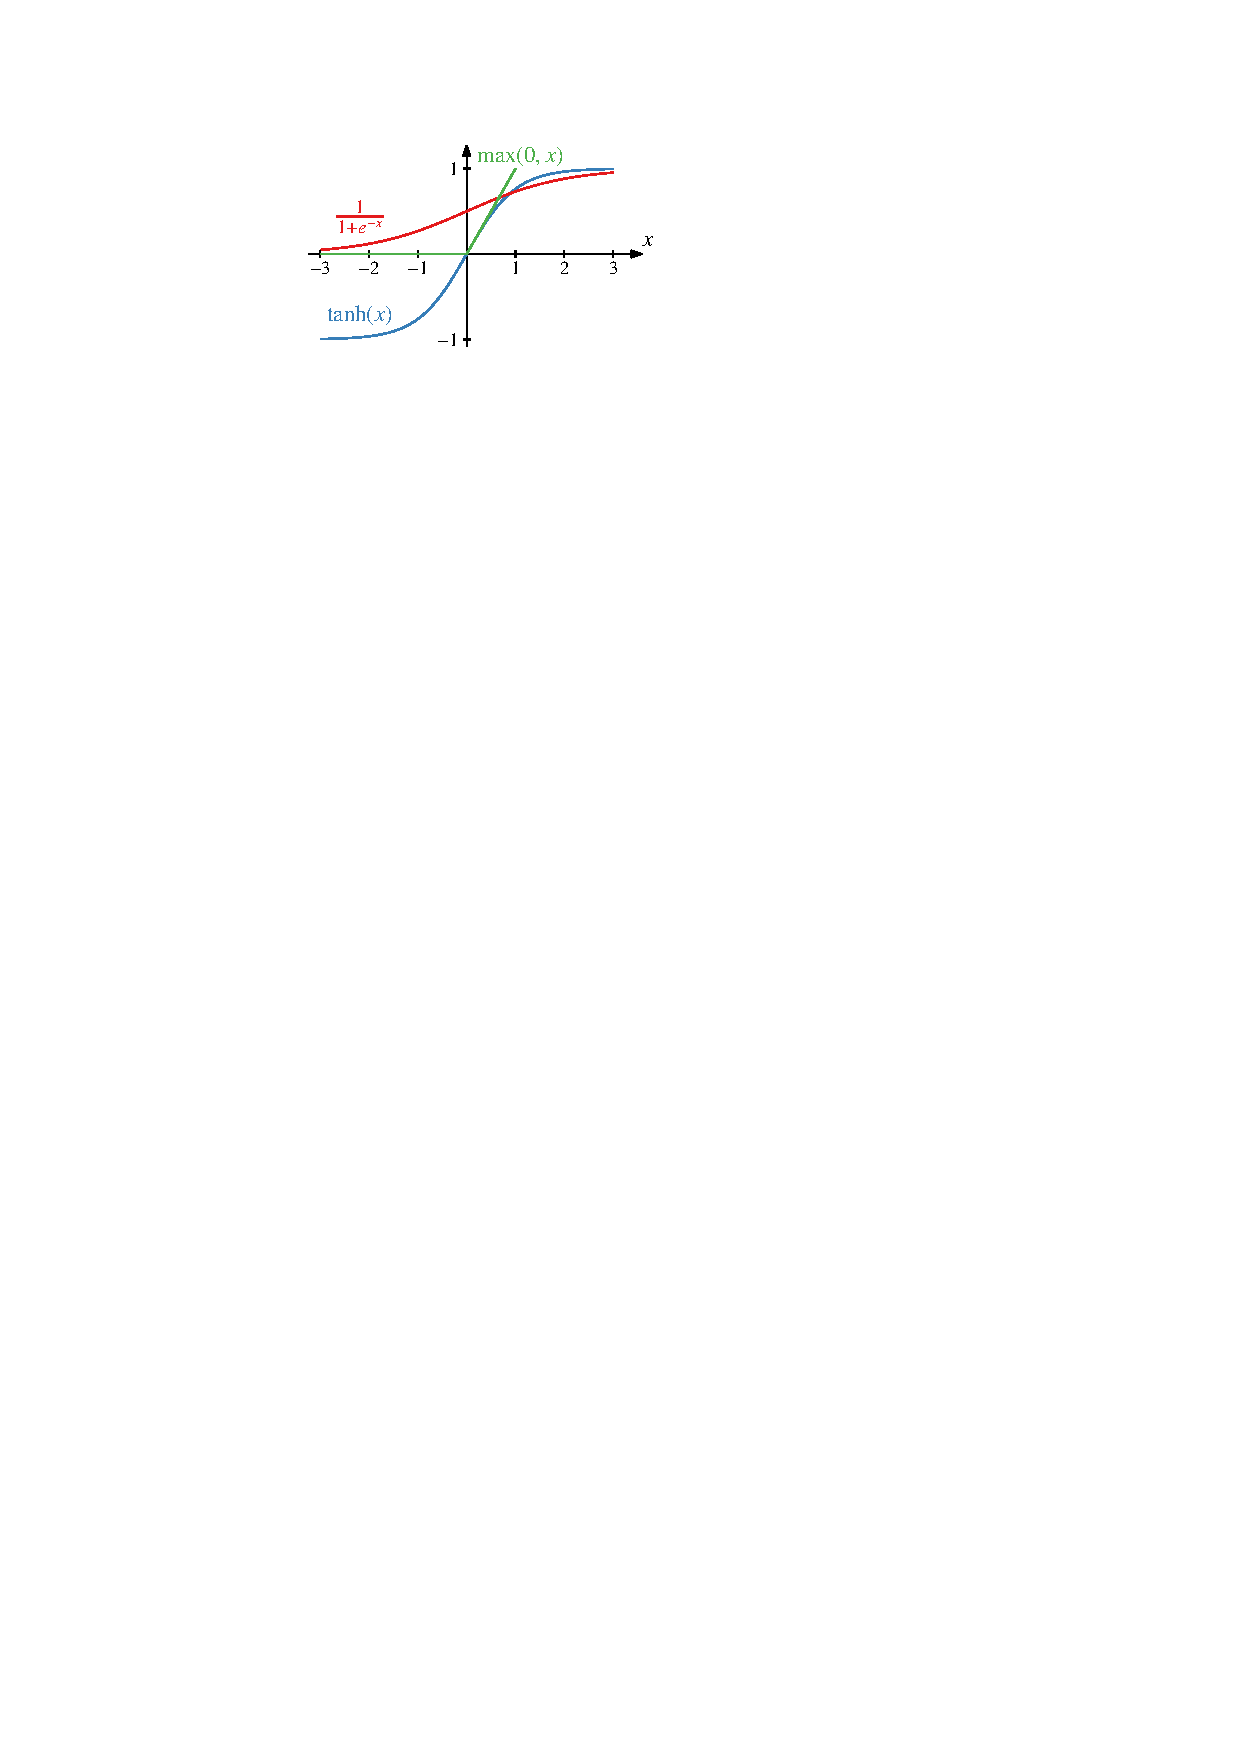
\includegraphics{./figures/theory/activation_functions.pdf}
    \captionof{figure}{Commonly used activation functions: logistic function (red),
      hyperbolic tangent (blue) and rectified linear unit (green).}
    \label{fig:activation_functions}
  \end{minipage}
\end{figure}
In Figure~\ref{fig:multi_layer_perceptron} a multi-layer perceptron with a
single hidden layer is shown. Two layers are connected by an affine
transformation and subsequent application of an element-wise, nonlinear and
differentiable activation function~$\bm{\varphi}$. These layers are called dense
or densely-connected layers, as each neuron is connected to every other neuron
in the neighboring layer. The weight of each connection between two neurons is
determined by weight matrices~$\mathbf{W}$.
% \begin{align*}
%   &\mathbf{h} = \bm{\varphi}_{\text{h}}(\mathbf{W}_{\text{hx}} \mathbf{x} + \mathbf{b}_{\text{h}})
%   &\mathbf{y} = \bm{\varphi}_{\text{y}}(\mathbf{W}_{\text{yh}} \mathbf{h} + \mathbf{b}_{\text{y}}) \eqcomma
% \end{align*}
The number of neurons in the hidden layers as well as activation functions are
hyperparameters (i.e.\ parameters that are set prior to training) of the model.
The sizes of the input and output layers are constrained by the number of input
variables and the number of desired outputs, respectively. Moreover the
activation function of the output layer is constrained by the underlying task.
For binary classification the logistic function
\begin{align*}
  \sigma(x) = \frac{1}{1 + e^{-x}}
\end{align*}
is applied to a single output neuron~$x$ giving the probability of an
observation being of the positive class (e.g.\ signal). For multi-class
classification the number of output neurons is chosen to equal the number of
classes to be distinguished and the \emph{softmax} function \cite{esl, bishop}
\begin{align*}
  \varphi_i(\mathbf{x}) = \frac{e^{x_i}}{\sum_j e^{x_j}}
\end{align*}
is chosen as the activation function, where~$\varphi_i(\mathbf{x})$ is the
activation of the $i$-th neuron and $x_i$ its value before activation. The
\emph{softmax} function ensures that the sum of all activations in a layer
equals to one, such that they can be interpreted as class probabilities.
Activation functions that are commonly used for the intermediate layers are
depicted in Figure~\ref{fig:activation_functions}.

Thus far neural networks are viewed as nonlinear parametric functions mapping
input variables~$\mathbf{x}$ to a response~$\mathbf{y}$ without regarding the
choice of parameters (i.e.\ weights and biases of each layer). The model
parameters are determined using gradient descent by minimising an objective
function (training of the model). The objective function penalises errors in the
predictions of the model and is commonly called the loss function. Categorical
cross-entropy is generally used for multi-class classification differentiating
between $K$~classes. For an observation belonging to a
class~$k \in \{1, \dots, K\}$ it is defined as \cite{esl, bishop}
\begin{align*}
  L\left(k, \mathbf{p}(\mathbf{x}) \right) = - \log\left( p_k(\mathbf{x}) \right) \eqcomma
\end{align*}
where~$\mathbf{p}(\mathbf{x}) = \mathbf{y}(\mathbf{x})$ is the probabilistic
interpretation of the model with class probabilities~$p_k$ (after \emph{softmax}
activation) and discriminating variables~$\mathbf{x}$. For binary classification
it is sufficient to give the predicted probability~$p$ for the positive class
such that the binary cross-entropy can be written as
\begin{align*}
  L(t, p(\mathbf{x})) = -t \, \log(p(\mathbf{x})) - (1 - t) \, \log(1 - p(\mathbf{x})) \eqcomma
\end{align*}
with the binary indicator~$t$ encoding the true class (0 for the negative and 1
for the positive class). For a subset of observations with weights~$w_i$ the
loss~$\mathcal{L}$ is defined as
\begin{align*}
  &\mathcal{L} = \frac{\sum_i w_i L_i}{\sum_j w_j}
    \qquad \text{with} \qquad
    L_i = L\left(k_i, \mathbf{p}(\mathbf{x}_i)\right) \eqdot
\end{align*}
In case of the cross-entropy $\mathcal{L}$ can be interpreted as the negative
log-likelihood of the network parameters given the observed subset of data and
assuming the distribution of classes follows a (generalised) \textsc{Bernoulli}
distribution \cite{bishop}.

The task of finding the parameters of the model minimising the expected loss
\todo{Maximising the likelihood} on a set of training data is solved using
stochastic gradient descent. This requires information on the gradient of the
loss~$\mathcal{L}(\bm{\theta})$ with respect to the model
parameters~$\bm{\theta}$ while keeping the training examples fixed. Each layer
in the computational graph making up the network has a well-defined derivative
such that by repeatedly applying the chain rule for partial derivatives the
gradient $\nabla_{\bm{\theta}} \mathcal{L}(\bm{\theta})$ can be calculated
symbolically. This procedure is generally known as error backpropagation or
\emph{BackProp} \cite{bishop, lecun-backprop}. Knowing the gradient of the loss
an iterative optimisation method called mini-batch stochastic\footnote{The
  gradient of the loss on the full training sample is approximated by the
  gradient on a mini-batch.} gradient descent is employed. Initially the weights
are randomised to small values and biases set to zero. The set of training
examples is divided into subsets of fixed size called mini-batches. In an
iterative procedure the parameters are updated according to
\begin{align*}
  \bm{\theta}_{t+1} = \bm{\theta}_t - \eta \, \nabla_{\bm{\theta}} \mathcal{L}(\bm{\theta}_t) \eqcomma
\end{align*}
where $\eta > 0$ is called the learning rate and
$\nabla_{\bm{\theta}} \mathcal{L}(\bm{\theta}_t)$ is the gradient evaluated on
the mini-batch. One pass over all mini-batches is called an epoch and typically
multiple epochs are required to train a model. In practice, the loss on an
independent validation set is observed and the procedure is stopped when the
validation loss stops decreasing.
% \todo[inline]{Find more references; Large penalties to predictions that are far
%   off; Perfect classifiers have loss of zero (can always be reached with complex
%   models); Cross validation?}

\subsection{Recurrent Neural Networks}
\label{sec:rnn_theory}
Events reconstructed in particle detectors can contain a variable number of
reconstructed objects of the same type e.g.\ particle tracks or clusters in the
calorimeter. The rigid structure of feedforward neural networks does not offer a
general method to classify events with variable numbers of objects. Recurrent
neural networks~(RNN) provide an approach to sequence classification by
introducing so called cyclical connections within layers in which units are
connected to themselves. These recurrent connections allow decisions to be made
in the context of the sequence (e.g.\ obeying constraints due to momentum
conservation) by making the network able to store information on previous
objects \cite{graves}.

The \textsc{Elman} network is introduced and will be extended to the long
short-term memory~(LSTM) architecture used in this thesis. Biases are omitted in
the following description as they can be absorbed into the weight matrices.

\subsubsection{Simple Recurrent Networks}
\label{sec:simple_recurrent_networks}
\begin{figure}[htb]
  \centering
  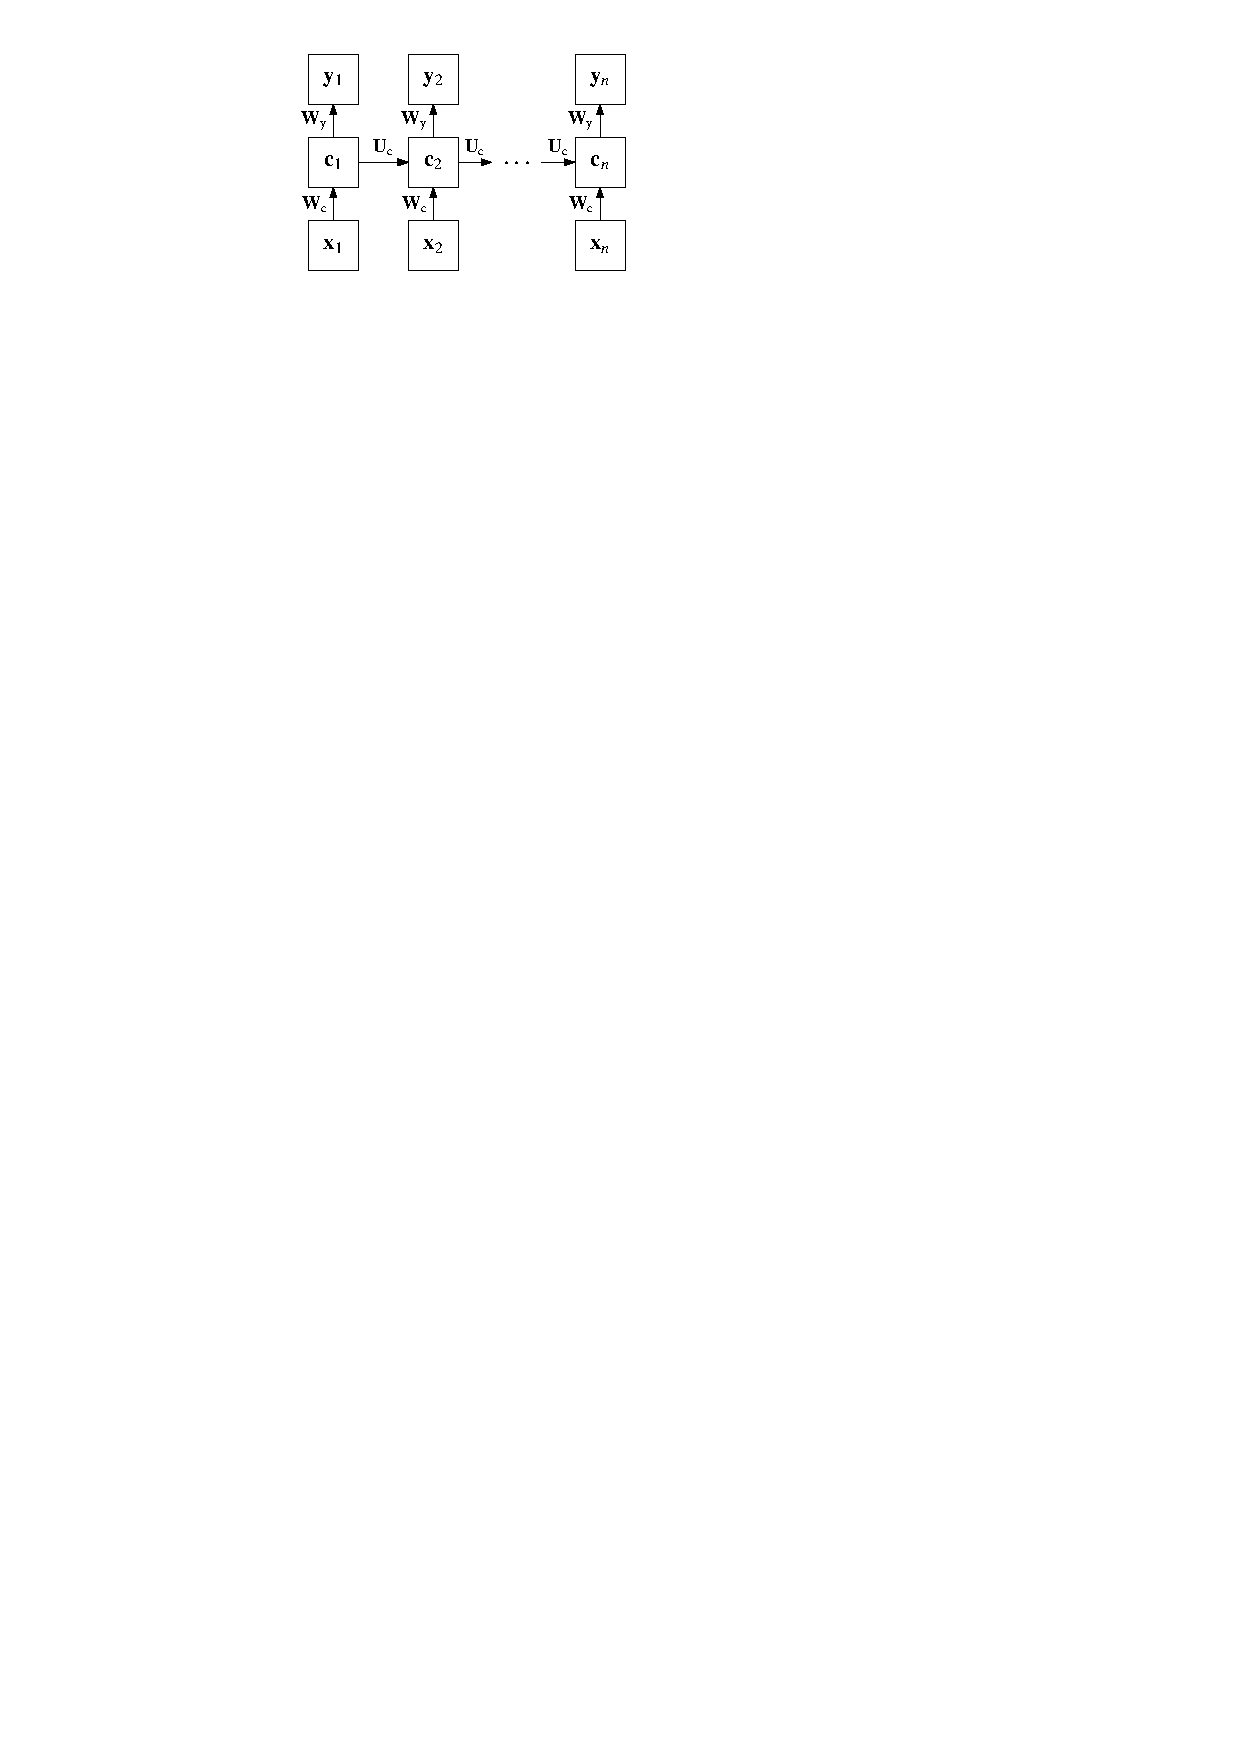
\includegraphics{./figures/theory/elman_rnn.pdf}
  \caption{\textsc{Elman} network in compact form with a recurrent connection
    and after unfolding the network in time. The black square indicates a delay
    of one time step. Applications of nonlinear activation functions are
    omitted. Adapted from Ref.~\cite{lecun_bengio_hinton_DL}.}
  \label{fig:schematic_elman_rnn}
  %\footnote{Nomenclature originates from RNNs being used to predict quantities as a function of time.}
\end{figure}

Recurrent neural networks are able to map a sequence of input variables to a
sequence of outputs. Both sequences can contain an arbitrary number of objects.
An example of a \emph{Simple Recurrent Network} is the \textsc{Elman}
network~\cite{elman} depicted in Figure~\ref{fig:schematic_elman_rnn}. After
unfolding the network in time it can be represented as a feedforward network
with weights shared between time steps. The input
sequence~$\left( \mathbf{x}_i \right)_{i=1}^n$ is processed one element at a
time. The sequence of cell states~$\mathbf{c}_t$ and outputs~$\mathbf{y}_t$ are
computed by iteratively applying the rule
\begin{align*}
  \mathbf{c}_t &= \bm{\varphi}_{\text{c}}\Big( \mathbf{W}_{\text{c}} \mathbf{x}_{t} + \mathbf{U}_{\text{c}} \mathbf{y}_{t-1} \Big)
  &\mathbf{y}_t &= \bm{\varphi}_{\text{y}}\Big( \mathbf{W}_{\text{y}} \mathbf{c}_{t} \Big)
\end{align*}
with weights~$\mathbf{W}$, recurrent weights~$\mathbf{U}$ and activation
functions~$\bm{\varphi}$, while incrementing the time step~$t$~\cite{elman,
  graves}. The initial cell state is often set to $\mathbf{c}_0 = \mathbf{0}$
but the particular choice can differ between implementations. All weights are
shared between time steps which allows sequences of arbitrary length to be
processed by the network. The cell state~$\mathbf{c}_t$ at each time step~$t$ is
updated using the external input~$\mathbf{x}_t$ as well as the cell
state~$\mathbf{c}_{t-1}$ of the previous time step forming the recurrent
connection. This allows a memory of previous inputs to persist in the internal
state of the network thus enabling the output~$\mathbf{y}_t$ to depend on the
history of the sequence. As Simple Recurrent Networks process the input sequence
in a predefined direction, only the past information can influence the output at
a specific time step making the order of the input sequence important. An
architecture allowing the context (past and future) to influence the output at a
given time~$t$ are so called bidirectional RNNs.

The evaluation of the gradient for the training process follows the same
principles used for feedforward neural networks but now also considering that
the chain rule has to be applied for each time step and one has to consider that
the weights between time steps are shared (\emph{backpropagation through
  time}~\cite{williams_zipser}). After unfolding the network in time the
training is analogous to that of feedforward neural networks.

In this thesis, RNNs are used for the classification of a sequence of
reconstructed objects in its entirety as opposed to classifying each element in
the sequence. For this task the full output sequence of the recurrent network is
not needed, such that only the output of the last time step is used. Simple
Recurrent Networks like the \textsc{Elman} network show that the gradient signal
decays with each time step making it difficult learn structure spanning over
multiple time steps in the input sequence. This is known as the \emph{vanishing
  gradient problem}~\cite{hochreiter, lecun_bengio_hinton_DL}. The following
section will present an extension to this architecture enabling the network to
learn long-term dependencies.
% \todo{This is due to the repeated
%   application of the activation function e.g.\ $\tanh$ in the recurrent
%   connection leading to a exponential decay of the gradient -- also affects
%   feedforward networks}.

\subsubsection{Long Short-Term Memory}
\label{sec:lstm}
The long short-term memory (LSTM) network developed in Ref.~\cite{lstm} solves
the \emph{vanishing gradient problem} by introducing multiplicative gates
\todo{define} that control the flow of information in the network. In
Figure~\ref{fig:schematic_lstm} a schematic depiction of an unfolded LSTM at
time~$t$ is shown.
\begin{figure}[htb]
  \centering
  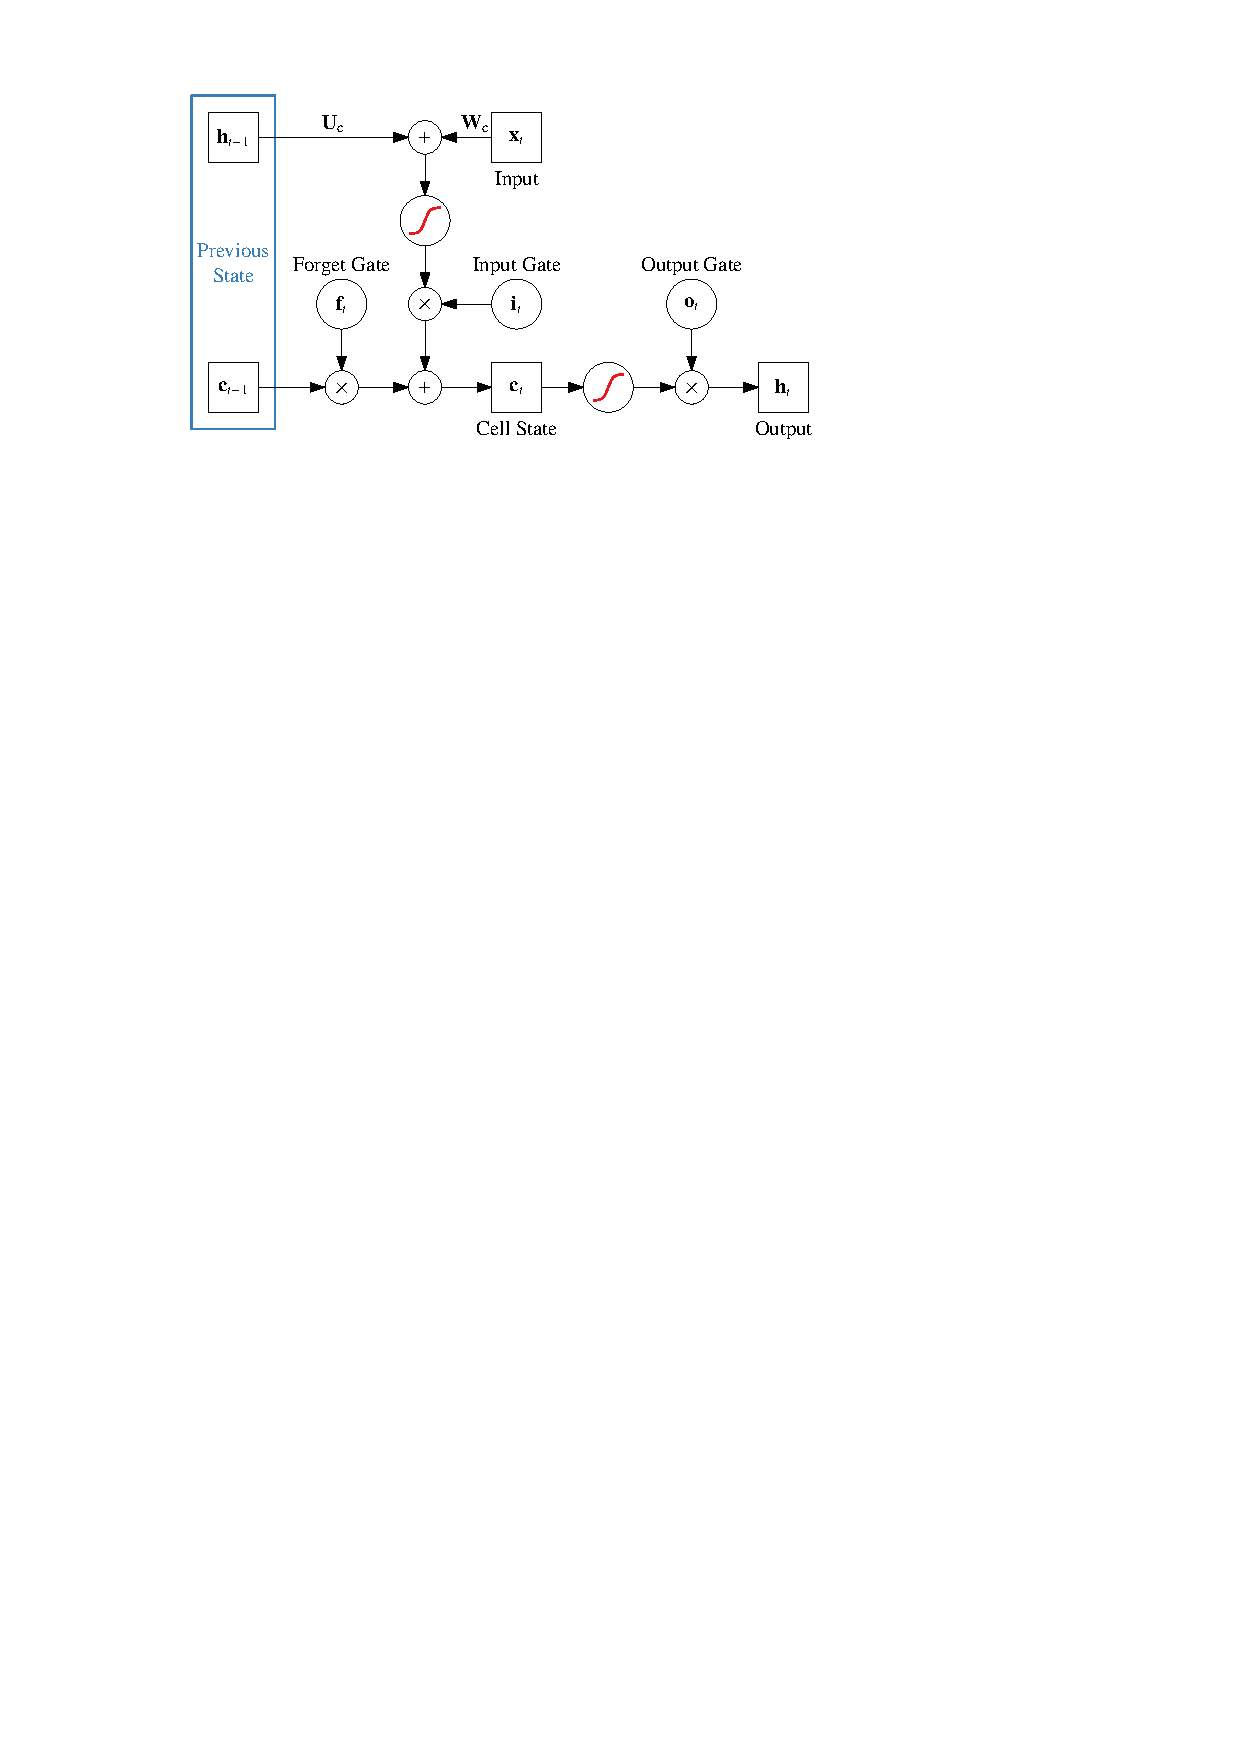
\includegraphics{./figures/theory/LSTM.pdf}
  \caption{LSTM-cell unfolded in time at a fixed time step~$t$. Nodes
    with~$\times$ ($+$) multiply (add) their inputs element-wise while ones
    containing a sigmoid shape apply a nonlinear activation function. The
    dependency of the gate vectors $\mathbf{i}_t$, $\mathbf{o}_t$ and
    $\mathbf{f}_t$ on input~$\mathbf{x}_t$ and output~$\mathbf{y}_{t-1}$ is
    omitted.}
  \label{fig:schematic_lstm}
\end{figure}
The LSTM represents a differentiable memory cell with three gates called the
input, output and forget gate. The gate vectors, controlling the information
flow, are given by \cite{goodfellow_dl, graves}
\begin{align*}
  \mathbf{i}_{t} &= \bm{\sigma}\left( \mathbf{W}_{\text{i}} \mathbf{x}_{t} + \mathbf{U}_{\text{i}} \mathbf{y}_{t-1} \right) &
  \mathbf{o}_{t} &= \bm{\sigma}\left( \mathbf{W}_{\text{o}} \mathbf{x}_{t} + \mathbf{U}_{\text{o}} \mathbf{y}_{t-1} \right) &
  \mathbf{f}_{t} &= \bm{\sigma}\left( \mathbf{W}_{\text{f}} \mathbf{x}_{t} + \mathbf{U}_{\text{f}} \mathbf{y}_{t-1} \right)
\end{align*}
with separate weights~$W$ and recurrent weights~$U$ for each gate. The
element-wise logistic function~$\bm{\sigma}$ is used to map the gate activations
into the interval $[0, 1]$. Notably the gate activations depend on the
input~$\mathbf{x}_t$ at time~$t$ as well as the output~$\mathbf{y}_{t-1}$ of the
LSTM at the previous time step. To understand how the gating controls the flow
of information in a LSTM one looks at the update of the cell state~$\mathbf{c}$
with each time step \cite{graves, goodfellow_dl}
\begin{align*}
  \mathbf{c}_{t} &= \mathbf{f}_{t} \circ \mathbf{c}_{t-1}
                   + \mathbf{i}_{t} \circ \bm{\varphi}_{\text{c}}(
                   \mathbf{W}_{\text{c}} \mathbf{x}_{t}+ \mathbf{U}_{\text{c}}
                   \mathbf{y}_{t-1} ) \eqcomma
\end{align*}
where $\circ$ denotes the element-wise product of two column vectors and the
activation function~$\bm{\varphi}_c$ is the hyperbolic tangent in the
implementation \cite{keras} used in this thesis. Similar to the Simple Recurrent
Networks the initial cell state $\mathbf{c}_0$ and output $\mathbf{y}_0$ are set
to $\mathbf{0}$. The input gate controls how much information from the
input~$\mathbf{x}_t$ and previous output~$\mathbf{y}_{t-1}$ is taken into the
cell state thereby reducing the inclusion of irrelevant information. A main
feature of the LSTM architecture is the direct connection of cell states between
two successive time steps via the forget gate which solves the \emph{vanishing
  gradient problem} \cite{lstm, graves}. The forget gate enables the network to
gradually reset its internal state once stored information has become
irrelevant. Finally the output~$\mathbf{y}_t$ is calculated using \cite{graves,
  goodfellow_dl}
\begin{align*}
  \mathbf{y}_{t} &= \mathbf{o}_{t} \circ \bm{\varphi}_{\text{y}}(\mathbf{c}_{t}) \eqcomma
\end{align*}
where~$\bm{\varphi}_\text{y}$ is the hyperbolic tangent. The activation of the
output gate determines how much of the cell state is presented at the output of
the network. Overall the multiplicative gating of the LSTM allows information to
persist in its internal state over a long period of time with gates resembling
the write, read and reset gates of conventional memory cells. Alternative
architectures to LSTMs exist (e.g.\ \emph{Gated Recurrent Units}) but were not
investigated in this thesis.

\section{Technical Setup}
\label{sec:tech_setup}

In this thesis the \emph{Toolkit for Multivariate Data
  Analysis}~(TMVA)~\cite{tmva} is used for the BDT-based studies on tau
identification in Chapter~\ref{sec:bdt}. This framework is extensively used for
evaluating multivariate algorithms for the reconstruction of hadronic tau lepton
decays in the ATLAS experiment.

The neural network based studies in chapters~\ref{sec:rnn}
and~\ref{sec:decaymode} use the \textsc{keras} framework~\cite{keras} which
offers implementations of commonly used layers (i.e.\ the rules to compute the
forward pass as well as the symbolic derivatives for backpropagation), loss
functions and optimisers. Moreover, it takes care of the necessary bookkeeping
when building neural networks. The \textsc{theano} backend~\cite{theano} is used
in \textsc{keras} performing fast computation of mathematical expressions for
training and evaluation of the networks. For the preprocessing of the data, the
\textsc{numpy} \cite{numpy} and \textsc{scipy} \cite{scipy} packages are used.
The training of the neural networks uses the \textsc{Adam} optimiser~\cite{adam}
which is a stochastic gradient descent algorithm with adaptive learning rates
offering quick convergence with little parameter tuning. The layers used in this
thesis are (using the \textsc{keras} naming convention):
Dense~(densely-connected layer), LSTM, Merge~(concatenates outputs from multiple
layers), and Masking~(skips inputs in recurrent networks filled with a
predefined default value). The dense and LSTM layers use biases which were
previously omitted.

%%% Local Variables:
%%% mode: latex
%%% TeX-master: "mythesis"
%%% End:
